\documentclass[a4paper]{article}

\usepackage[italian]{babel}
\usepackage[utf8]{inputenc}
\usepackage{graphicx}
\usepackage{hyperref}

\begin{document}

\title{Risoluzione del problema STSP tramite metodo esatto e metaeuristica, comparazione}
%\subtitle{Relazione Progetto del corso di Metodi e Modelli per lOttimizzazione Combinatoria}
\author{Carlo Maria Massimo 1058513}
\date{\today}
\maketitle

\tableofcontents

    \section{Introduzione}
        Il lavoro in oggetto si propone lo scopo di valutare attraverso alcune sperimentazioni la bont\`a di metodi
        di risoluzione del problema STSP tramite metaeuristica rispetto a pi\`u collaudati metodi esatti.
        I metodi che sfruttano le metaeuristiche e qualche forma di ricerca locale sono spesso utilizzati per le migliori
        performance in termini di rapidit\`a di calcolo ed uso delle risorse, a fronte di un possibile degrado nella qualit\`a
        dei risultati forniti in output.

        In questo lavoro \`e stata implementata una ricerca tramite modello PLI e risolutore CPLEX e tramite algoritmo genetico.

    \section{Implementazione}
        L'implementazione della ricerca tramite metodo esatto \`e stata realizzata prendendo spunto da un'esercitazione di laboratorio
        relativa ad un problema di ATSP ed implementando in pratica il modello descritto nella consegna dell'esercitazione 1.

        L'implementazione della ricerca tramite algoritmo genetico \`e stata realizzata partendo dalla descrizione dei passi
        sulle dispense del corso, cercando per quanto possibile di introdurre qualche elemento di originalit\`a e di miglioramento rispetto
        allo schema standard dell'algoritmo proposto.

        \subsection{Note}
        Durante gli esperimenti entrambe le ricerche partono da un'istanza del problema comune, modellata nella classe \emph{Instance}.
        L'istanza rappresenta il grafo dei punti che dovranno essere effettuati sulla piastra.
        In particolare \`e descritta da:

        \begin{enumerate}
            \item cardinalit\`a dell'insieme dei nodi del grafo
            \item dimensioni della piastra (limite alle coordinate dei punti)
            \item il nodo di partenza
            \item la matrice delle distanze tra i nodi
            \item la lista dei nodi (identificati dalle proprie coordinate nello spazio 2D)
        \end{enumerate}

        La classe \emph{Model} racchiude il modello e la ricerca tramite PLI mentre le classi \emph{Solution}, \emph{Population} e \emph{Solver}
        implementano l'algoritmo genetico.
        
    \section{Risoluzione tramite modello PLI}
        Per risolvere il problema tramite modello di programmazione lineare intera mista si \`e ricorsi alla modellazione dello stesso come problema di
        rete di flusso e si \`e utilizzato il risolutore CPLEX per la ricerca di una soluzione ottima.
        Il modello implementato \`e quello fornito nell'esercitazione 1, la verifica della correttezza \`e stata fatta mediante ispezione del file
        \emph{stsp.lp} generato dal risolutore.

    \section{Risoluzione tramite algoritmo genetico}
        L'algoritmo implementato segue il seguente schema:
        \begin{enumerate}
            \item codifica delle soluzioni del problema;
            \item inizializzazione di una popolazione iniziale;
            \item ripetizione fino al soddisfacimento di condizioni di arresto:
                \begin{enumerate}
                    \item seleziona coppie di parent dalla popolazione corrente;
                    \item ricombina i parent generando due figli per ogni coppia;
                    \item rinnova la popolazione corrente selezionado nuovi individui
                        tra i figli appena generati, sulla base della misura di fitness;
                \end{enumerate}
            \item restituisci la soluzione migliore generata.
        \end{enumerate}

        \subsection{Parametri e calibrazione}
            Tutti i paramtri sono stati calibrati a mano per mancanza di tempo anche se sarebbe stato preferibile un approccio di tipo
            \emph{grid search}.
            I parametri che determinano una variazione nella condotta della ricerca con metaeuristica sono essenzialmente due:
            \begin{itemize}
                \item $accept\_prob$ ovvero un valore di probabilit\`a che determina:
                    \begin{itemize}
                        \item l'accettazione di nuove soluzioni generate per ricombinazione;
                        \item l'applicazione della mutazione per inversione invece della rottura / riparazione della soluzione
                    \end{itemize}
                    Questo parametro varia tra i valori $0.99$ in fase di intensificazione e $0.90$ in fase di diversificazione.
                \item $hc\_iterations$ che determina il numero di iterazioni massime nella ricerca locale; durante le fasi di
                    intensificazione assume il valore $0$ (iterazioni illimitate), mentre in fase di diversificazione assume il valore 3.
            \end{itemize}

            Vi \`e poi il parametro $max\_tot\_iterations$ che gestisce il massimo numero di popolazioni generabili dall'algoritmo ed \`e fissato
            ad $N*5$ dove $N$ \`e la cardinalit\`a dell'insieme dei nodi del grafo.

            Il parametro $iterations\_without\_improvement$ decide il limite di iterazioni improduttive oltre il quale passare dalla
            fase di intensificazione alla fase di diversificazione ed \`e fissato ad $N*2$.

            La dimensione della popolazione \`e stato arbitrariamente fissato a 10 individui.

        \subsection{Codifica delle soluzioni}
            La codifica delle soluzioni adottata \`e quella detta ``path representation'', ovvero
            ogni soluzione \`e rappresentata da un vettore di interi (\emph{sequence}) che contiene
            gli indici del vettore dei nodi del grafo. L'ordine rappresentato nel vettore determina il cammino.
            Ogni indice appare solo una volta nel vettore \emph{sequence} e questo fa si che si riesca a modellare
            un ciclo Hamiltoniano.

        \subsection{Inizializzazione della popolazione iniziale}
            La popolazione di partenza viene inizialmente generata in maniera casuale. La met\`a di questa popolazione
            viene migliorata tramite una ricerca locale tramite \emph{Hill Climbing} che pu\`o essere o meno limitata
            nel numero di iterazioni dal fatto che si sia scelto di iniziare diversificando o intensificando la ricerca.
            La ricerca locale si basa su un vicinato 2-opt.

        \subsection{Selezione genitori}
            La fase di selezione degli individui per la ricombinazione procede selezionando dalla popolazione un certo numero
            (fissato) di coppie di individui distinti.
            La selezione avviene tramite la tecnica detta ``Fitness proportionate selection'', basandosi su una misura di \emph{fitness}
            definita come segue:

            $$f_i = (1 / e_i) - ic_i - hc_i$$

            dove:
            \begin{itemize}
                \item $e_i$ \`e il valore della funzione obiettivo sulla soluzione i-esima;
                \item $ic_i$ \`e il coefficiente di inammissibilit\`a definito proporzionalmente
                    al numero di ripetizioni nel vettore degli indici;
                \item $hc_i$ \`e il coefficiente di somiglianza con l'ottimo corrente definito proporzionalmente
                    all'inverso della distanza di Hamming con l'ottimo corrente se questa \`e maggiore di 0, un valore
                    fissato altrimenti.
            \end{itemize}

            Vengono create tante coppie quante sono gli individui di una popolazione.
        
        \subsection{Ricombinazione degli individui selezionati}
            Le coppie di individui parent cos\`i individuati vengono ricombinati tra di loro utilizzando l'operatore detto
            ``order-crossover''.

            Inizialmente si era optato per un operatore ``cut-point'' con $k$ punti di taglio definiti casualmente e variabili
            in numero tra una coppia e l'altra.
            Questo operatore \`e stato presto abbandonato in favore dell'``order-crossover'' in quanto causava un netto e veloce
            peggioramento delle soluzioni generate principalmente perch\'e estremamente inammissibili.

            Data l'inerente fragilit\`a di una soluzione nei confronti di operatori di ricombinazione insensibili rispetto ai nodi
            risultanti dalla ricombinazione si \`e preferito utilizzare l'operatore ``order-crossover'' che preserva l'ammissibilit\`a
            della soluzione generata rispetto ai genitori.

            Ogni nuova soluzione generata tramite ricombinazione, se ammissibile viene accettata con probabilit\`a $accept\_prob$,
            se inammissibile viene scartata con uguale probabilit\`a.
            Da questa procedura risulta una progenie di cardinalit\`a doppia rispetto a quella di una popolazione regolare.

            Gli individui di questo insieme vengono quindi sottoposti a mutazione ed in seguito a training.

            \subsubsection{Mutazione}
                Ogni individuo della progenie viene sottoposto, con probabilit\`a $accept\_prob$ ad un operatore di ``mutazione per inversione''.
                Nel caso in cui non gli venga applicato tale operatore l'individuo viene mutato comunque ma secondo il seguente schema:
                \begin{itemize}
                    \item se ammissibile: un gene selezionato casualmente viene impostato ad un valore casuale tra i possibili valori degli indici,
                        risultando quindi potenzialmente nella perdit\`a di ammissibilit\`a;
                    \item se inammissibile: viene ``riparato'', ovvero ogni ripetizione di indice viene sostituita con uno degli indici mancanti in maniera ordinata,
                        ripristinando l'ammissibilit\`a.
                \end{itemize}

                Si noti come questa secondo tipo di mutazione incida decisamente di pi\`u in fase di diversificazione in quanto $accept\_prob$ diminuisce.

            \subsubsection{Training}
                Conseguentemente alla fase di mutazione gli individui vengono migliorati tramite la stessa ricerca locale utilizzata per inizializzare
                la popolazione iniziale (\emph{Hill Climbing}).

                Anche in questo caso le iterazioni che l'algoritmo esegue sono limitate o meno a seconda che ci si trovi in fase di diversificazione o di intesificazione.

        \subsection{Rinnovamento della popolazione}
            Gli individui cos\`i manipolati vengono sottoposti quindi a selezione tramite ``Fitness proportionate selection'' fino a coprire la
            cardinalit\`a degli individui di una popolazione.

            La popolazione cos\`i ottenuta diviene la nuova generazione.
            
            Viene quindi confrontata la miglior soluzione della nuova generazione con l'ottimo corrente e se i criteri di arresto sono soddisfatti viene ritornata la migliore delle due soluzioni,
            altrimenti si procede con un'altra iterazione.
\newpage
    \section{Risultati delle simulazioni}
        
        \subsection{Esperimenti}
        I parametri degli esperimenti (indicati con \textbf{Ei}) effettuati sono stati i seguenti:
        \begin{description}
            \item[E1] insieme dei nodi di cardinalit\`a 10--70 con step 10, inizializzazione casuale dei punti e dimensioni di piastra fissate (500x500);
            \item[E2] insieme dei nodi di cardinalit\`a 10--70 con step 10, inizializzazione casuale dei punti e dimensioni di piastra crescenti: 100x100--700x700;
            \item[E3] come \textbf{E1} ma partendo con una fase di intensificazione invece che diversificazione;
            \item[E4] insieme dei nodi di cardinalit\`a 10--70 con step 10, inizializzazione dei punti su una circonferenza e dimensioni di piastra fissate (500x500).
            \item[E5] insieme dei nodi di cardinalit\`a 100, inizializzazione casuale dei punti e dimensioni di piastra fissate (500x500).
        \end{description}

        \subsection{Risultati}
            Seguono i risultati ottenuti dalle simulazioni effettuate.
            \subsubsection{Ricerca con metodo esatto}

                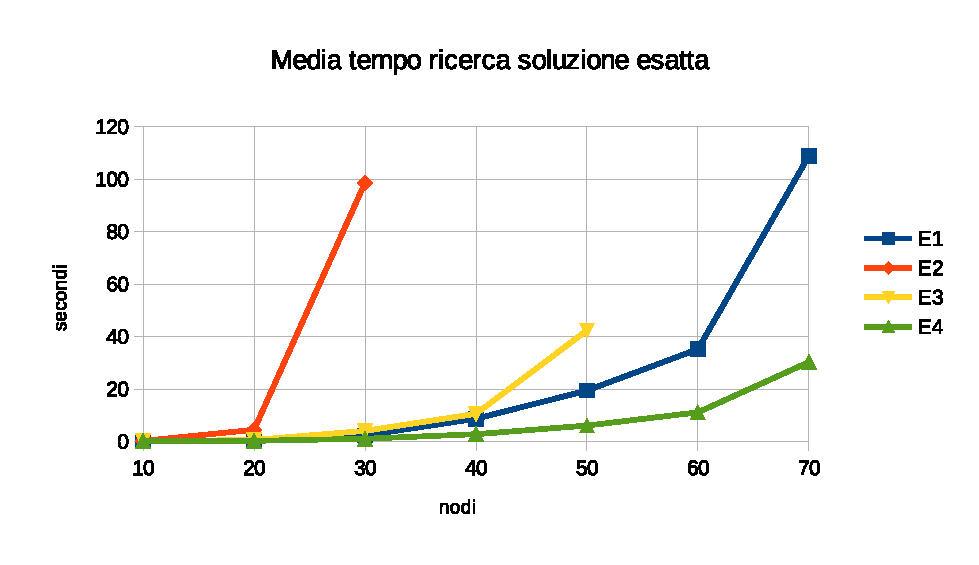
\includegraphics[scale=0.7]{img/exavgtime}

                Si nota una crescita esponenziale all'aumentare della dimensione del problema.

                Il valore molto elevato che si riscontra in \textbf{E4} rispetto agli altri esperimenti \`e probabilmente dovuto all'assenza di un controllo di collisione
                nella generazione dei punti sulla circonferenza, complicando di molto il lavoro della fase di Branch and Bound.

                \textbf{E5} si attesta su $1454.63$ secondi.

                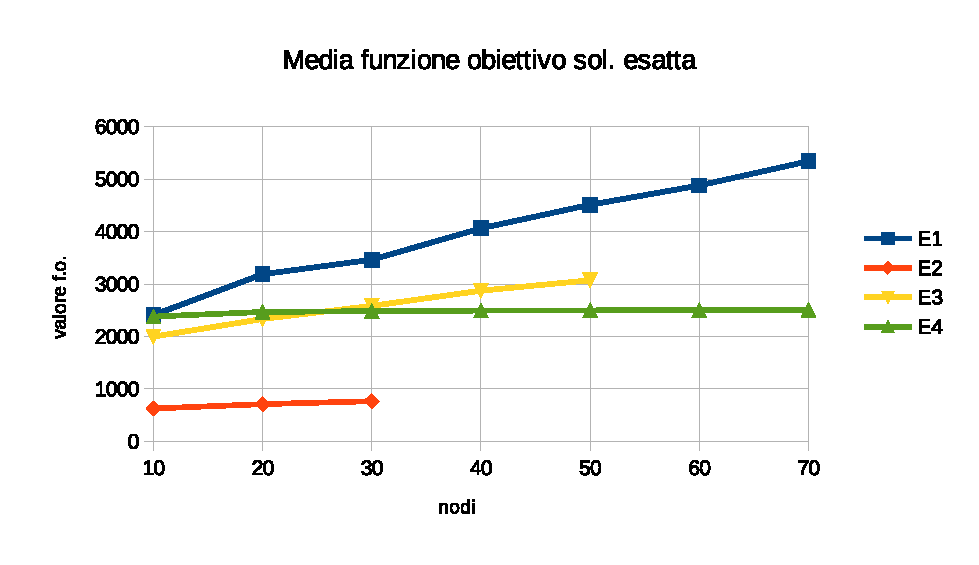
\includegraphics[scale=0.7]{img/exavgobj}

                I valori alti in \textbf{E2} sono dovuti all'espansione dell'area della piastra mentre quelli molto bassi in \textbf{E4} alla
                conformazione del grafo (circonferenza).

                Valore in \textbf{E5}: $4001.42$.

            \subsubsection{Ricerca con metaeuristica}

                    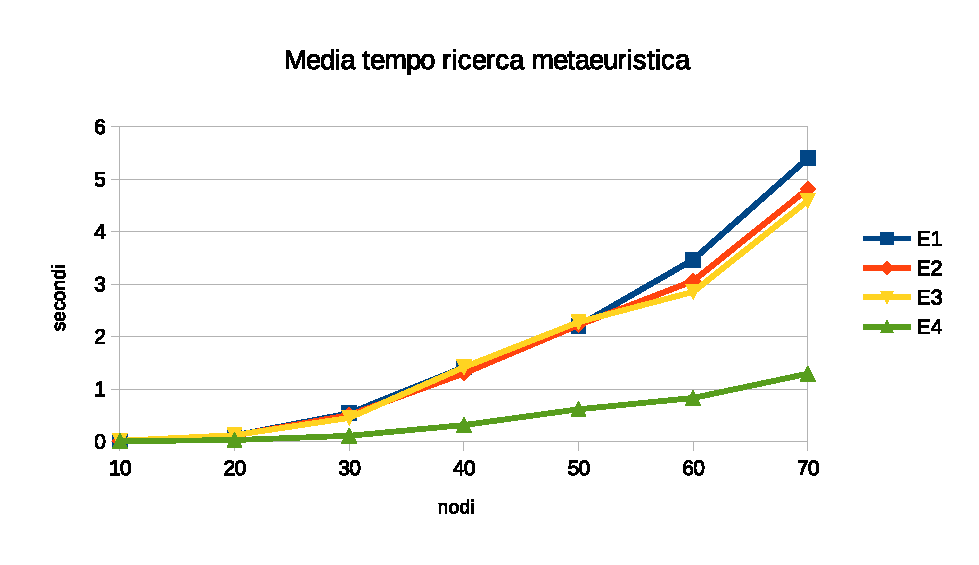
\includegraphics[scale=0.7]{img/gavgtime}

                    Come si pu\`o notare i valori sono estremamente pi\`u contenuti rispetto alla ricerca esatta, anche per problemi di dimensioni
                    considerevoli.

                    Tempo impiegato in \textbf{E5}: $12.3757$ secondi.

                    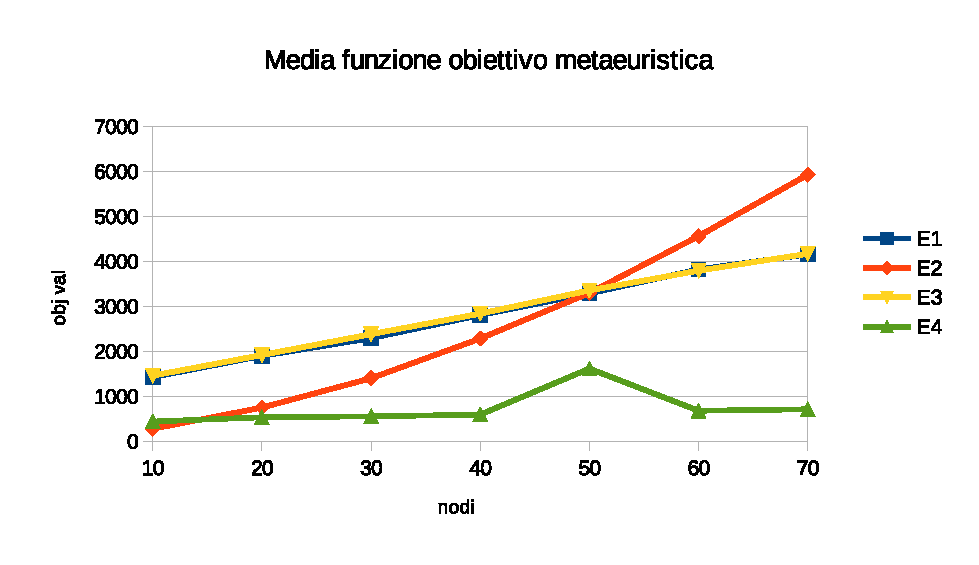
\includegraphics[scale=0.7]{img/gavgobj}

                    La perdita di performance rispetto all'ottimalit\`a rimane perlopi\`u contenuta.

                    Aumentando anche di un solo ordine di grandezza il numero di iterazioni massime permesse all'algoritmo si otteneva un discreto
                    avvicinamento ai valori della soluzione ottima, andando per\`o ad incidere considerevolmente sui tempi di esecuzione per i problemi
                    di dimensione pi\`u modesta.

                    Valore in \textbf{E5}: $5683.34$ a partire da un valore nella popolazione iniziale di $23367.6$.

                    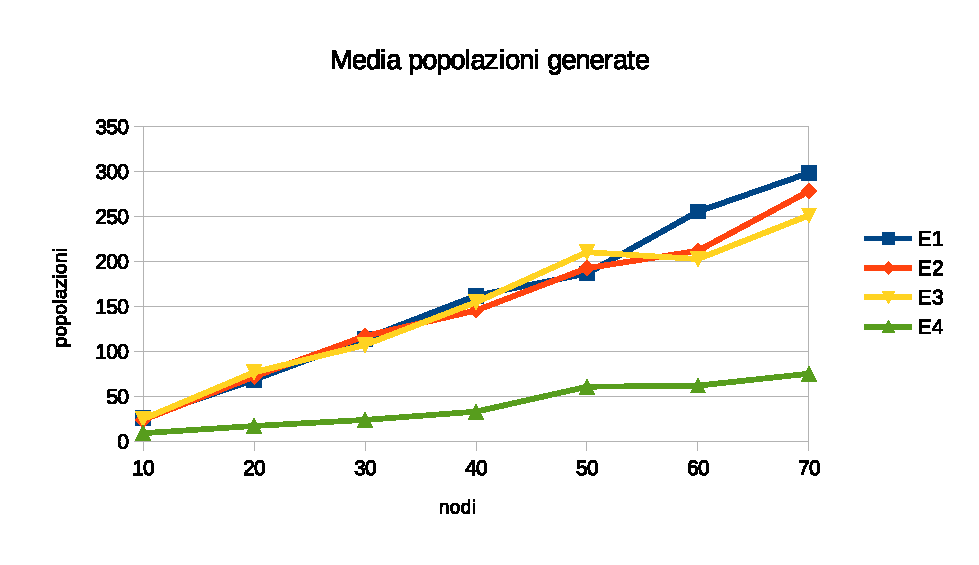
\includegraphics[scale=0.7]{img/popavg}

                    Si noti come la scarsa complessit\`a del problema in \textbf{E4} influisca drasticamente sul numero di iterazioni necessarie per raggiungere
                    una soluzione stabile.

                    In \textbf{E5}: 428 popolazioni in media.

                \subsubsection{Comparazione}

                    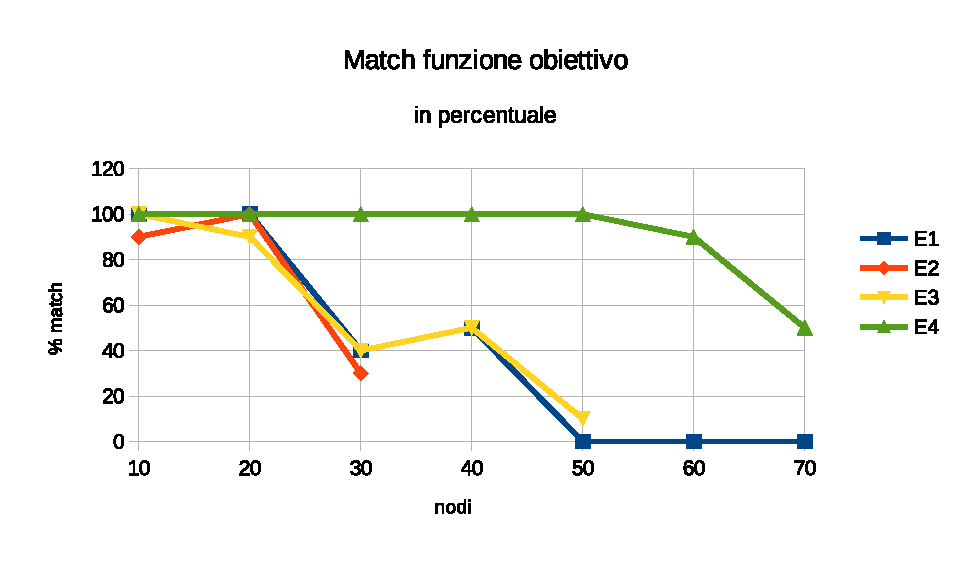
\includegraphics[scale=0.7]{img/match}

                    La ricerca con metaeuristica si comporta in maniera sostanzialmente identica alla ricerca con metodo esatto per dimensioni di problema modeste,
                    decrescendo nel numero di match man mano che il problema diviene pi\`u complesso.
                    
                    Come detto in precedenza si sono notati sostanziali miglioramenti per grafi con molti nodi aumentando il numero massimo di nuove generazioni permesse, a discapito per\`o
                    del tempo di esecuzione nel caso di problemi pi\`u semplici.

                    In \textbf{E5} non si \`e verificato match.

                    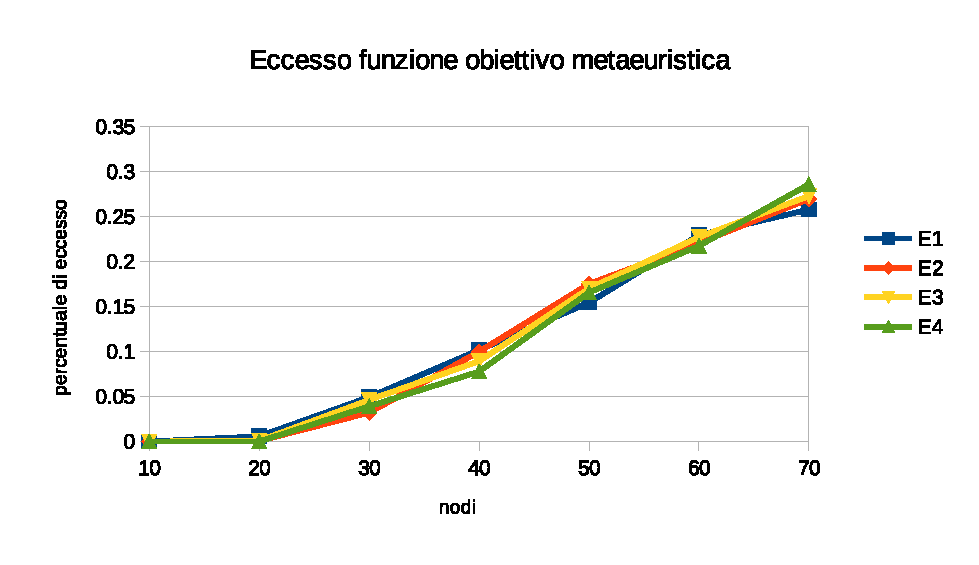
\includegraphics[scale=0.7]{img/excess}

                    Da questo grafico si pu\`o notare che la discrepanza nei risultati tra le due ricerche cresce abbastanza linearmente
                    con l'aumentare della complessit\`a del problema.
                    Il valore massimo rimane sempre comunque sotto il $30\%$.


                    In \textbf{E5} l'eccesso \`e del $42\%$.

    \section{Conclusioni}
        STSP \`e un problema inerentemente molto complesso, che nel caso esatto richiede moltissimo sforzo.
        La ricerca nel caso esatto \`e inoltre piuttosto sensibile alla conformazione del problema, come involontariamente esemplificato
        dall'esperimento \textbf{E4}, mentre per contro la ricerca tramite metaeuristica sembra essere meno influenzata dalla struttura del grafo,
        a meno di casi estremamente particolari (la circonferenza di \textbf{E4} appunto).

        Con questo lavoro si \`e visto, non senza sorpresa, che \`e possibile raggiungere un buon grado di approssimazione rispetto ad una
        soluzione ottima, con tempi di esecuzione estremamente ridotti.

        \`E opinione dell'autore che un fine-tuning dei parametri di ricerca con adeguata strategia \emph{grid search} possa dare risultati
        ancora migliori rispetto a quelli esposti in questo documento.

\end{document}
